\section{Objetivo}\label{objetivo}

Nuestro objetivo será desarrollar un cliente para Twitter que sea capaz
de mostrar en una pantalla LCD el último tuit de la cuenta
@esibot en tiempo real.

\subsection{Componentes del sistema}\label{componentes-del-sistema}

\subsubsection{LCD}\label{lcd}

Usaremos una panel PCD8544 es un panel LCD de resolución 84x48 monocromático que fue usado en
  varios modelos de Nokia, como el 5110. Hay disponibles librerís para
  varias plataformas con las que se puede escribir formas y texto de
  forma sencilla., el que se utilizaba en los nokia 5110.

En esta pantalla imprimiremos el último tuit de la cuenta @esibot con el siguiente formato:

\begin{verbatim}
@ESIBot 18:57 el 5/10/2015
Hoy han comenzado las actividades para este curso con el
1er seminario de conceptos básicos. Mañana repetimos, de
16 a 18 en la 110 ;)
\end{verbatim}

\subsubsection{Arduino UNO}\label{arduino-uno}

Será el encargado de recibir los tuits enviados por la \emph{Raspberry
Pi} y mostrarlos en el panel LCD usando la librería pertinente.

Sus funciones principales son:

\begin{itemize}
\item
  Estar a la escucha de tuits enviados por la \emph{Raspberry Pi}.
\item
  Cuando reciba un nuevo tuit, mostrarlo en el panel LCD.
\end{itemize}

\subsubsection{Raspberry PI}\label{raspberry-pi}

Será la encargada de consultar la cuenta @esibot y cuando encuentre un nuevo
mensaje lo enviará al Arduino para que lo muestre en el panel LCD. Dado
que es el elemento de la red que está conectado a Internet, necesitaremos un
\emph{dongle} \emph{WiFi} o un cable \emph{Ethernet} y que tenga una conexión
configurada correctamente.

\subsection{Protocolos}\label{protocolos}

Puesto que vamos a conectar diferentes dispositivos entre sí, vamos a
necesitar unos protocolos que nos faciliten la comunicación.

\subsubsection{Bluetooth}\label{bluetooth}

\begin{figure}[h]
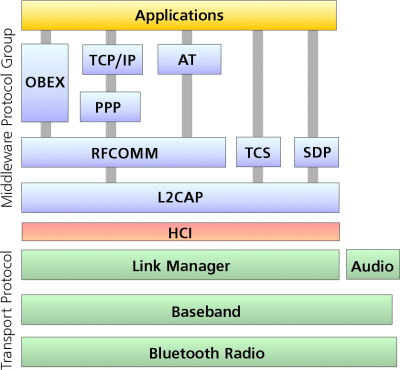
\includegraphics[width=0.5\textwidth]{fig01}
\centering
\caption{Stack de Bluetooth}
\end{figure}

Entre las diferentes posibilidades elegimos \emph{Bluetooth} porque es
de los protocolos más usados y fáciles de usar. Con \emph{Bluetooth}
cubriremos desde la capa física hasta la capa de transporte del modelo
OSI.

Sin embargo, el dispositivo que usaremos nos permite emular un puerto
serie, es decir, que nosotros lo conectaremos a la UART de nuestos
dispositivos (\emph{Arduino} y \emph{Raspberry Pi}) y será como si
estuviesen conectados por puerto serie. Esto nos facilitará muchísimo la
conexión.

\subsubsection{MQTT-SN}\label{mqtt-sn}

MQTT-SN (MQTT for Sensors Networks) es un protocolo de nivel de aplicación \textbf{simple}
y \textbf{ligero} que nos permite crear un \emph{broker} donde se
conecten múltiples clientes. Estos clientes pueden enviar mensajes al
\emph{broker} o \textbf{suscribirse a un topic}. Está basado en el
protocolo MQTT, pero ha sido simplificado para ser usado en sensores (No
implementa todo el \emph{stack} IP). Nosotros lo usaremos sobre
\emph{Bluetooth} que, como ya hemos visto, para nosotros será como tener
un puerto serie virtual.

\begin{figure}[h]
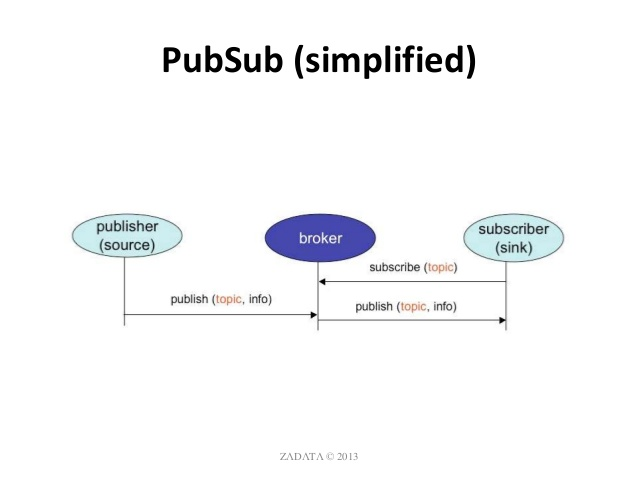
\includegraphics[width=\textwidth]{fig02}
\centering
\caption{Comunicación mediante MQTT}
\end{figure}

El funcionamiento de este protocolo encaja perfectamente con lo que
nosotros queremos hacer. Instalaremos un \emph{broker} en la
\emph{Raspberry Pi} y desarrollaremos usando \emph{Python} un
\emph{publisher} que correrá también en la \emph{Raspberry Pi}.

Mientras tanto, en el \emph{Arduino} tendremos un \emph{suscriber} que
se suscribirá a un \emph{topic}. Nótese que podría haber varios
\emph{Arduinos} conectados a la misma Raspberry, aunque tendríamos que
tener un dispositivo \emph{Bluetooth} en la \emph{Raspberry Pi} por cada
\emph{Arduino}.